% Options for packages loaded elsewhere
\PassOptionsToPackage{unicode}{hyperref}
\PassOptionsToPackage{hyphens}{url}
\PassOptionsToPackage{dvipsnames,svgnames,x11names}{xcolor}
%
\documentclass[
]{article}
\usepackage{amsmath,amssymb}
\usepackage{iftex}
\ifPDFTeX
  \usepackage[T1]{fontenc}
  \usepackage[utf8]{inputenc}
  \usepackage{textcomp} % provide euro and other symbols
\else % if luatex or xetex
  \usepackage{unicode-math} % this also loads fontspec
  \defaultfontfeatures{Scale=MatchLowercase}
  \defaultfontfeatures[\rmfamily]{Ligatures=TeX,Scale=1}
\fi
\usepackage{lmodern}
\ifPDFTeX\else
  % xetex/luatex font selection
\fi
% Use upquote if available, for straight quotes in verbatim environments
\IfFileExists{upquote.sty}{\usepackage{upquote}}{}
\IfFileExists{microtype.sty}{% use microtype if available
  \usepackage[]{microtype}
  \UseMicrotypeSet[protrusion]{basicmath} % disable protrusion for tt fonts
}{}
\makeatletter
\@ifundefined{KOMAClassName}{% if non-KOMA class
  \IfFileExists{parskip.sty}{%
    \usepackage{parskip}
  }{% else
    \setlength{\parindent}{0pt}
    \setlength{\parskip}{6pt plus 2pt minus 1pt}}
}{% if KOMA class
  \KOMAoptions{parskip=half}}
\makeatother
\usepackage{xcolor}
\usepackage[margin=1in]{geometry}
\usepackage{color}
\usepackage{fancyvrb}
\newcommand{\VerbBar}{|}
\newcommand{\VERB}{\Verb[commandchars=\\\{\}]}
\DefineVerbatimEnvironment{Highlighting}{Verbatim}{commandchars=\\\{\}}
% Add ',fontsize=\small' for more characters per line
\usepackage{framed}
\definecolor{shadecolor}{RGB}{248,248,248}
\newenvironment{Shaded}{\begin{snugshade}}{\end{snugshade}}
\newcommand{\AlertTok}[1]{\textcolor[rgb]{0.94,0.16,0.16}{#1}}
\newcommand{\AnnotationTok}[1]{\textcolor[rgb]{0.56,0.35,0.01}{\textbf{\textit{#1}}}}
\newcommand{\AttributeTok}[1]{\textcolor[rgb]{0.13,0.29,0.53}{#1}}
\newcommand{\BaseNTok}[1]{\textcolor[rgb]{0.00,0.00,0.81}{#1}}
\newcommand{\BuiltInTok}[1]{#1}
\newcommand{\CharTok}[1]{\textcolor[rgb]{0.31,0.60,0.02}{#1}}
\newcommand{\CommentTok}[1]{\textcolor[rgb]{0.56,0.35,0.01}{\textit{#1}}}
\newcommand{\CommentVarTok}[1]{\textcolor[rgb]{0.56,0.35,0.01}{\textbf{\textit{#1}}}}
\newcommand{\ConstantTok}[1]{\textcolor[rgb]{0.56,0.35,0.01}{#1}}
\newcommand{\ControlFlowTok}[1]{\textcolor[rgb]{0.13,0.29,0.53}{\textbf{#1}}}
\newcommand{\DataTypeTok}[1]{\textcolor[rgb]{0.13,0.29,0.53}{#1}}
\newcommand{\DecValTok}[1]{\textcolor[rgb]{0.00,0.00,0.81}{#1}}
\newcommand{\DocumentationTok}[1]{\textcolor[rgb]{0.56,0.35,0.01}{\textbf{\textit{#1}}}}
\newcommand{\ErrorTok}[1]{\textcolor[rgb]{0.64,0.00,0.00}{\textbf{#1}}}
\newcommand{\ExtensionTok}[1]{#1}
\newcommand{\FloatTok}[1]{\textcolor[rgb]{0.00,0.00,0.81}{#1}}
\newcommand{\FunctionTok}[1]{\textcolor[rgb]{0.13,0.29,0.53}{\textbf{#1}}}
\newcommand{\ImportTok}[1]{#1}
\newcommand{\InformationTok}[1]{\textcolor[rgb]{0.56,0.35,0.01}{\textbf{\textit{#1}}}}
\newcommand{\KeywordTok}[1]{\textcolor[rgb]{0.13,0.29,0.53}{\textbf{#1}}}
\newcommand{\NormalTok}[1]{#1}
\newcommand{\OperatorTok}[1]{\textcolor[rgb]{0.81,0.36,0.00}{\textbf{#1}}}
\newcommand{\OtherTok}[1]{\textcolor[rgb]{0.56,0.35,0.01}{#1}}
\newcommand{\PreprocessorTok}[1]{\textcolor[rgb]{0.56,0.35,0.01}{\textit{#1}}}
\newcommand{\RegionMarkerTok}[1]{#1}
\newcommand{\SpecialCharTok}[1]{\textcolor[rgb]{0.81,0.36,0.00}{\textbf{#1}}}
\newcommand{\SpecialStringTok}[1]{\textcolor[rgb]{0.31,0.60,0.02}{#1}}
\newcommand{\StringTok}[1]{\textcolor[rgb]{0.31,0.60,0.02}{#1}}
\newcommand{\VariableTok}[1]{\textcolor[rgb]{0.00,0.00,0.00}{#1}}
\newcommand{\VerbatimStringTok}[1]{\textcolor[rgb]{0.31,0.60,0.02}{#1}}
\newcommand{\WarningTok}[1]{\textcolor[rgb]{0.56,0.35,0.01}{\textbf{\textit{#1}}}}
\usepackage{longtable,booktabs,array}
\usepackage{calc} % for calculating minipage widths
% Correct order of tables after \paragraph or \subparagraph
\usepackage{etoolbox}
\makeatletter
\patchcmd\longtable{\par}{\if@noskipsec\mbox{}\fi\par}{}{}
\makeatother
% Allow footnotes in longtable head/foot
\IfFileExists{footnotehyper.sty}{\usepackage{footnotehyper}}{\usepackage{footnote}}
\makesavenoteenv{longtable}
\usepackage{graphicx}
\makeatletter
\def\maxwidth{\ifdim\Gin@nat@width>\linewidth\linewidth\else\Gin@nat@width\fi}
\def\maxheight{\ifdim\Gin@nat@height>\textheight\textheight\else\Gin@nat@height\fi}
\makeatother
% Scale images if necessary, so that they will not overflow the page
% margins by default, and it is still possible to overwrite the defaults
% using explicit options in \includegraphics[width, height, ...]{}
\setkeys{Gin}{width=\maxwidth,height=\maxheight,keepaspectratio}
% Set default figure placement to htbp
\makeatletter
\def\fps@figure{htbp}
\makeatother
\setlength{\emergencystretch}{3em} % prevent overfull lines
\providecommand{\tightlist}{%
  \setlength{\itemsep}{0pt}\setlength{\parskip}{0pt}}
\setcounter{secnumdepth}{5}
\usepackage{fontspec}
\setmainfont{Times New Roman}
\usepackage{longtable}
\usepackage{pdflscape}
\usepackage{booktabs}
\usepackage{longtable}
\usepackage{array}
\usepackage{multirow}
\usepackage{wrapfig}
\usepackage{float}
\usepackage{colortbl}
\usepackage{pdflscape}
\usepackage{tabu}
\usepackage{threeparttable}
\usepackage{threeparttablex}
\usepackage[normalem]{ulem}
\usepackage{makecell}
\usepackage{xcolor}
\ifLuaTeX
  \usepackage{selnolig}  % disable illegal ligatures
\fi
\usepackage{bookmark}
\IfFileExists{xurl.sty}{\usepackage{xurl}}{} % add URL line breaks if available
\urlstyle{same}
\hypersetup{
  pdftitle={Churn Management},
  pdfauthor={Giovanni Compiani},
  colorlinks=true,
  linkcolor={Maroon},
  filecolor={Maroon},
  citecolor={Blue},
  urlcolor={blue},
  pdfcreator={LaTeX via pandoc}}

\title{Churn Management}
\author{Giovanni Compiani}
\date{}

\begin{document}
\maketitle

{
\hypersetup{linkcolor=}
\setcounter{tocdepth}{2}
\tableofcontents
}
\setlength{\parskip}{6pt}
\newpage

\begin{Shaded}
\begin{Highlighting}[]
\FunctionTok{library}\NormalTok{(bit64)}
\FunctionTok{library}\NormalTok{(data.table)}
\FunctionTok{library}\NormalTok{(ggplot2)}
\FunctionTok{library}\NormalTok{(broom)}
\FunctionTok{library}\NormalTok{(knitr)}
\FunctionTok{library}\NormalTok{(dplyr)}
\FunctionTok{library}\NormalTok{(kableExtra)}
\end{Highlighting}
\end{Shaded}

\section{Overview}\label{overview}

Cell2Cell, a wireless telecommunications company (with its name altered
for confidentiality), is working to reduce customer churn. The objective
of this project is to create a model that predicts customer churn at
Cell2Cell and to leverage insights from the model to design a targeted
incentive strategy aimed at decreasing churn rates.

In the assignment, you will address these key issues:

\begin{enumerate}
\def\labelenumi{\arabic{enumi}.}
\item
  Is customer churn at Cell2Cell predictable from the customer
  information that Cell2Cell maintains?
\item
  What factors drive customer churn? Which factors are particularly
  important?
\item
  What incentives should Cell2Cell offer to prevent customer churn?
\item
  What is the economic value of a proposed targeted plan to prevent
  churn, and how does this value differ across customer segments?
  Compare the economic value to an incentive with a cost of \$100 and
  another incentive with a cost of \$175. Which customers segments
  should receive the incentive? Does the answer depend on the success
  probability?
\end{enumerate}

Note that, in what follows, the key steps you need to take are
highlighted in \emph{italic}.

\newpage

\section{Data}\label{data}

All data are contained in the file \texttt{Cell2Cell.RData}, which is
posted on Canvas.

\begin{Shaded}
\begin{Highlighting}[]
\NormalTok{data\_folder    }\OtherTok{=} \StringTok{"./Data"}
\NormalTok{Cell2Cell }\OtherTok{=} \StringTok{"Cell2Cell.RData"}
\FunctionTok{load}\NormalTok{(}\FunctionTok{paste0}\NormalTok{(data\_folder, }\StringTok{"/"}\NormalTok{, Cell2Cell))}
\end{Highlighting}
\end{Shaded}

\medskip

Please consult the file \texttt{Cell2Cell-Database-Documentation.xlsx}
for a description of the data and some summary statistics. Note that
\emph{calibration sample} is an alternative term for \emph{training} or
\emph{estimation} sample.

\emph{Report the churn rate in the calibration sample and in the
validation sample and compare the two.}

\begin{Shaded}
\begin{Highlighting}[]
\CommentTok{\# str(cell2cell\_DT)}

\NormalTok{calibration\_sample }\OtherTok{\textless{}{-}} \FunctionTok{subset}\NormalTok{(cell2cell\_DT, calibrat }\SpecialCharTok{==} \DecValTok{1}\NormalTok{)}
\NormalTok{validation\_sample }\OtherTok{\textless{}{-}} \FunctionTok{subset}\NormalTok{(cell2cell\_DT, calibrat }\SpecialCharTok{==} \DecValTok{0}\NormalTok{)}

\CommentTok{\# Calculate churn rate in the calibration sample}
\NormalTok{calibration\_churn\_rate }\OtherTok{\textless{}{-}} \FunctionTok{mean}\NormalTok{(calibration\_sample}\SpecialCharTok{$}\NormalTok{churn)}
\FunctionTok{cat}\NormalTok{(}\StringTok{"Churn Rate in Calibration Sample:"}\NormalTok{, calibration\_churn\_rate, }\StringTok{"}\SpecialCharTok{\textbackslash{}n}\StringTok{"}\NormalTok{)}
\end{Highlighting}
\end{Shaded}

\begin{verbatim}
Churn Rate in Calibration Sample: 0.5 
\end{verbatim}

\begin{Shaded}
\begin{Highlighting}[]
\CommentTok{\# Calculate churn rate in the validation sample}
\NormalTok{validation\_churn\_rate }\OtherTok{\textless{}{-}} \FunctionTok{mean}\NormalTok{(validation\_sample}\SpecialCharTok{$}\NormalTok{churn)}
\FunctionTok{cat}\NormalTok{(}\StringTok{"Churn Rate in Validation Sample:"}\NormalTok{, validation\_churn\_rate, }\StringTok{"}\SpecialCharTok{\textbackslash{}n}\StringTok{"}\NormalTok{)}
\end{Highlighting}
\end{Shaded}

\begin{verbatim}
Churn Rate in Validation Sample: 0.01961542 
\end{verbatim}

\begin{Shaded}
\begin{Highlighting}[]
\CommentTok{\# Compare churn rates}
\ControlFlowTok{if}\NormalTok{ (calibration\_churn\_rate }\SpecialCharTok{\textgreater{}}\NormalTok{ validation\_churn\_rate) \{}
  \FunctionTok{cat}\NormalTok{(}\StringTok{"The churn rate is higher in the calibration sample.}\SpecialCharTok{\textbackslash{}n}\StringTok{"}\NormalTok{)}
\NormalTok{\} }\ControlFlowTok{else} \ControlFlowTok{if}\NormalTok{ (calibration\_churn\_rate }\SpecialCharTok{\textless{}}\NormalTok{ validation\_churn\_rate) \{}
  \FunctionTok{cat}\NormalTok{(}\StringTok{"The churn rate is higher in the validation sample.}\SpecialCharTok{\textbackslash{}n}\StringTok{"}\NormalTok{)}
\NormalTok{\} }\ControlFlowTok{else}\NormalTok{ \{}
  \FunctionTok{cat}\NormalTok{(}\StringTok{"The churn rates are the same in both samples.}\SpecialCharTok{\textbackslash{}n}\StringTok{"}\NormalTok{)}
\NormalTok{\}}
\end{Highlighting}
\end{Shaded}

\begin{verbatim}
The churn rate is higher in the calibration sample.
\end{verbatim}

You can see that the calibration sample was selected using
\emph{oversampling}. The purpose of oversampling was to obtain more
precise estimates (lower standard errors) when estimating a logistic
regression model. The validation sample, on the other hand, was not
created using oversampling and represents the \emph{true churn rate} in
the data.

As you can see, some variables have missing values, which---as you know
by now---is common and of no concern (unless the missing values indicate
some \emph{systematic} flaws or bias in how the data were constructed).
Most estimation methods in R will automatically delete rows with missing
values before estimating the model. However, the \texttt{predict}
methods will yield \texttt{NA} values if a row in the data used for
prediction contains missing values. Hence, in a situation where you
don't need to keep the full data I recommend to remove any observations
with missing values before you conduct the main analysis.

\emph{Perform this data-cleaning step.}

\begin{Shaded}
\begin{Highlighting}[]
\CommentTok{\# Remove rows with missing values from the data}
\NormalTok{cell2cell\_clean }\OtherTok{\textless{}{-}} \FunctionTok{na.omit}\NormalTok{(cell2cell\_DT)}

\CommentTok{\# Verify that missing values have been removed}
\FunctionTok{print}\NormalTok{(}\FunctionTok{sprintf}\NormalTok{(}\StringTok{"Original dataset had \%d rows"}\NormalTok{, }\FunctionTok{nrow}\NormalTok{(cell2cell\_DT)))}
\end{Highlighting}
\end{Shaded}

\begin{verbatim}
[1] "Original dataset had 71047 rows"
\end{verbatim}

\begin{Shaded}
\begin{Highlighting}[]
\FunctionTok{print}\NormalTok{(}\FunctionTok{sprintf}\NormalTok{(}\StringTok{"Cleaned dataset has \%d rows"}\NormalTok{, }\FunctionTok{nrow}\NormalTok{(cell2cell\_clean)))}
\end{Highlighting}
\end{Shaded}

\begin{verbatim}
[1] "Cleaned dataset has 69309 rows"
\end{verbatim}

\begin{Shaded}
\begin{Highlighting}[]
\FunctionTok{print}\NormalTok{(}\FunctionTok{sprintf}\NormalTok{(}\StringTok{"Removed \%d rows with missing values"}\NormalTok{, }\FunctionTok{nrow}\NormalTok{(cell2cell\_DT) }\SpecialCharTok{{-}} \FunctionTok{nrow}\NormalTok{(cell2cell\_clean)))}
\end{Highlighting}
\end{Shaded}

\begin{verbatim}
[1] "Removed 1738 rows with missing values"
\end{verbatim}

\newpage

\section{Model estimation}\label{model-estimation}

\emph{Estimate a logit model to predict the conditional churn
probability.}

\begin{Shaded}
\begin{Highlighting}[]
\CommentTok{\# Fit the logistic regression model}
\NormalTok{fit }\OtherTok{\textless{}{-}} \FunctionTok{glm}\NormalTok{(churn }\SpecialCharTok{\textasciitilde{}}\NormalTok{ ., }
             \AttributeTok{data =}\NormalTok{ cell2cell\_clean[, .SD, }\AttributeTok{.SDcols =} \SpecialCharTok{!}\FunctionTok{c}\NormalTok{(}\StringTok{"customer"}\NormalTok{, }\StringTok{"calibrat"}\NormalTok{)], }
             \AttributeTok{family =} \FunctionTok{binomial}\NormalTok{())}
\end{Highlighting}
\end{Shaded}

You can inspect the regression output using methods you already used,
such as \texttt{summary}. Having said this, especially when you have a
large number of inputs, it can be convenient to store the regression
estimates in a table. A simple way to do this is to install the
\href{https://cran.r-project.org/web/packages/broom/vignettes/broom.html}{broom
package} that has the purpose of cleaning up messy R output.

Using the \texttt{tidy} function in the \texttt{broom} package it is
trivial to capture the regression output in the form of a data.table:

\begin{Shaded}
\begin{Highlighting}[]
\CommentTok{\# Tidy the model output and convert to data.table}
\NormalTok{results\_DT }\OtherTok{\textless{}{-}} \FunctionTok{as.data.table}\NormalTok{(}\FunctionTok{tidy}\NormalTok{(fit))}

\CommentTok{\# Display the regression results with 5 decimal places}
\FunctionTok{kable}\NormalTok{(results\_DT, }\AttributeTok{digits =} \DecValTok{5}\NormalTok{)}
\end{Highlighting}
\end{Shaded}

\begin{longtable}[]{@{}lrrrr@{}}
\toprule\noalign{}
term & estimate & std.error & statistic & p.value \\
\midrule\noalign{}
\endhead
\bottomrule\noalign{}
\endlastfoot
(Intercept) & -0.82035 & 0.07826 & -10.48202 & 0.00000 \\
revenue & 0.00160 & 0.00066 & 2.42628 & 0.01525 \\
mou & -0.00028 & 0.00004 & -6.57237 & 0.00000 \\
recchrge & -0.00263 & 0.00074 & -3.55962 & 0.00037 \\
directas & 0.00023 & 0.00477 & 0.04781 & 0.96187 \\
overage & 0.00087 & 0.00023 & 3.73561 & 0.00019 \\
roam & 0.00281 & 0.00120 & 2.34317 & 0.01912 \\
changem & -0.00057 & 0.00005 & -12.57609 & 0.00000 \\
changer & 0.00290 & 0.00030 & 9.62096 & 0.00000 \\
dropvce & 0.00801 & 0.00698 & 1.14770 & 0.25109 \\
blckvce & 0.00345 & 0.00692 & 0.49930 & 0.61757 \\
unansvce & 0.00082 & 0.00037 & 2.23354 & 0.02551 \\
custcare & -0.00650 & 0.00230 & -2.82186 & 0.00477 \\
threeway & -0.03574 & 0.00969 & -3.68748 & 0.00023 \\
mourec & 0.00016 & 0.00011 & 1.39133 & 0.16413 \\
outcalls & 0.00056 & 0.00049 & 1.14705 & 0.25136 \\
incalls & -0.00178 & 0.00090 & -1.97778 & 0.04795 \\
peakvce & -0.00063 & 0.00018 & -3.41461 & 0.00064 \\
opeakvce & -0.00018 & 0.00022 & -0.82605 & 0.40878 \\
dropblk & -0.00015 & 0.00683 & -0.02230 & 0.98221 \\
callfwdv & -0.01786 & 0.02199 & -0.81229 & 0.41663 \\
callwait & -0.00008 & 0.00258 & -0.03224 & 0.97428 \\
months & -0.02227 & 0.00168 & -13.24110 & 0.00000 \\
uniqsubs & 0.17910 & 0.01576 & 11.36467 & 0.00000 \\
actvsubs & -0.18508 & 0.02251 & -8.22308 & 0.00000 \\
phones & 0.04958 & 0.01494 & 3.31785 & 0.00091 \\
models & 0.01377 & 0.02321 & 0.59341 & 0.55290 \\
eqpdays & 0.00142 & 0.00006 & 23.00599 & 0.00000 \\
age1 & -0.00409 & 0.00072 & -5.69500 & 0.00000 \\
age2 & -0.00093 & 0.00056 & -1.65423 & 0.09808 \\
children & 0.10973 & 0.02330 & 4.71042 & 0.00000 \\
credita & -0.17827 & 0.02964 & -6.01401 & 0.00000 \\
creditaa & -0.39057 & 0.02924 & -13.35695 & 0.00000 \\
prizmrur & 0.12196 & 0.04067 & 2.99893 & 0.00271 \\
prizmub & -0.03453 & 0.02019 & -1.71005 & 0.08726 \\
prizmtwn & 0.04801 & 0.02580 & 1.86104 & 0.06274 \\
refurb & 0.25268 & 0.02617 & 9.65444 & 0.00000 \\
webcap & -0.13360 & 0.03013 & -4.43361 & 0.00001 \\
truck & 0.03195 & 0.02968 & 1.07643 & 0.28173 \\
rv & 0.01306 & 0.03957 & 0.33005 & 0.74136 \\
occprof & -0.01636 & 0.02689 & -0.60840 & 0.54292 \\
occcler & 0.08278 & 0.06123 & 1.35196 & 0.17639 \\
occcrft & -0.02871 & 0.05222 & -0.54977 & 0.58248 \\
occstud & 0.07535 & 0.09816 & 0.76766 & 0.44269 \\
occhmkr & 0.11401 & 0.14800 & 0.77031 & 0.44112 \\
occret & -0.05320 & 0.07590 & -0.70091 & 0.48336 \\
occself & -0.01679 & 0.06743 & -0.24896 & 0.80339 \\
ownrent & 0.04038 & 0.03541 & 1.14025 & 0.25418 \\
marryun & 0.09073 & 0.02811 & 3.22759 & 0.00125 \\
marryyes & 0.05576 & 0.02686 & 2.07578 & 0.03791 \\
mailord & -0.04646 & 0.07135 & -0.65115 & 0.51495 \\
mailres & -0.09220 & 0.07162 & -1.28725 & 0.19801 \\
mailflag & 0.01346 & 0.07106 & 0.18935 & 0.84982 \\
travel & 0.00532 & 0.03914 & 0.13598 & 0.89184 \\
pcown & 0.02450 & 0.02556 & 0.95851 & 0.33781 \\
creditcd & 0.08633 & 0.03585 & 2.40792 & 0.01604 \\
retcalls & 0.18640 & 0.14799 & 1.25950 & 0.20785 \\
retaccpt & -0.17696 & 0.08357 & -2.11759 & 0.03421 \\
newcelly & -0.03518 & 0.02261 & -1.55586 & 0.11974 \\
newcelln & 0.02663 & 0.02596 & 1.02601 & 0.30489 \\
refer & -0.08079 & 0.03543 & -2.28011 & 0.02260 \\
incmiss & -0.07086 & 0.04938 & -1.43484 & 0.15133 \\
income & -0.00712 & 0.00499 & -1.42673 & 0.15366 \\
mcycle & 0.09062 & 0.07317 & 1.23859 & 0.21550 \\
setprcm & -0.09003 & 0.03317 & -2.71375 & 0.00665 \\
setprc & 0.00047 & 0.00023 & 1.99417 & 0.04613 \\
retcall & 0.64385 & 0.15547 & 4.14117 & 0.00003 \\
\end{longtable}

For \texttt{kable} to work, you need to load the \texttt{knitr} library.

\newpage

\section{Prediction: Accounting for
oversampling}\label{prediction-accounting-for-oversampling}

The idea of oversampling is as follows. If the response rate in the data
is small, there is a strong imbalance between observations with a
response of \(Y=1\) and a response of \(Y=0\). As a consequence,
estimating the model is difficult and the estimates will be imprecise,
i.e.~they will have large standard errors.

The solution: Create a training sample with one half of observations
randomly chosen from the original data with response \(Y=1\), and the
other half randomly chosen from the original data with response \(Y=0\).
Now estimation is easier and the standard errors will be smaller.

However, when applied to logistic regression, oversampling will result
in an inconsistent estimate of the intercept (constant) term, although
all other estimates will be consistent. Hence, if we do not de-bias
(adjust) the intercept, the predicted probabilities will be too large,
reflecting the artificial response rate of \(\frac{1}{2}\) in the
over-sampled training data.

In order to de-bias the scale of the predicted response (in this
example: churn) in the validation sample we need to supply an
\emph{offset variable} to the logistic regression model. An offset is a
known number that is added to the right-hand side of the regression when
estimating the model, and adding the offset will correspondingly change
the estimate of the intercept. The offset takes the form:
\[\text{offset}=\left[\log(\bar{p}_{t})-\log(1-\bar{p}_{t})\right]-\left[\log(\bar{p}_{v})-\log(1-\bar{p}_{v})\right]\]

Here, \(\bar{p}_{t}\) is the average response rate in the training
sample and \(\bar{p}_{v}\) is the average response rate in the
validation sample. Note that the offset is positive (given that
\(\bar{p}_t > \bar{p}_v\)), so that including the offset term when
estimating the model accounts for the fact that the training sample has
a higher share of \(Y=1\) relative to the validation sample.

Conversely, when we predict the response rate in the validation sample,
we set the offset variable to 0.

Why does this work? --- Conceptually, logistic regression is a
regression model for the log-odds of the response (outcome) probability,
\[\log \left(\frac{p}{1-p}\right) = \log(p) - \log(1-p) = \beta_0 + \beta_1 X_1 + \beta_2 X_1 + \dots \]

When we add the offset variable to the right hand side of the regression
model the estimation algorithm will ``incorporate'' the offset in the
intercept, \(\beta_0\). The effect of setting the offset to 0 (when
applying the model to the validation sample) is equivalent to
subtracting the offset from the intercept. Subtracting the offset
amounts to:

\begin{enumerate}
\def\labelenumi{(\roman{enumi})}
\item
  Subtracting \(\log(\bar{p}_{t})-\log(1-\bar{p}_{t})\), the log-odds of
  the artificial response rate in the training sample, and
\item
  Adding \(\log(\bar{p}_{v})-\log(1-\bar{p}_{v})\), the log-odds in the
  validation sample that reflects the true log-odds in the data.
\end{enumerate}

This process de-biases the predicted response, i.e.~restores the correct
response level in the validation sample.

Note: Never use over-sampling to create the validation sample, otherwise
the offset variable approach will not work.

\bigskip

\emph{Create an \texttt{offset\_var} variable and add it to the data
set. Then re-estimate the logistic regression. To tell \texttt{glm} that
you want to use \texttt{offset\_var}, you need to use a formula of the
form:}

\begin{Shaded}
\begin{Highlighting}[]
\NormalTok{y }\SpecialCharTok{\textasciitilde{}} \FunctionTok{offset}\NormalTok{(offset\_var) }\SpecialCharTok{+} \ErrorTok{\textless{}}\NormalTok{all other variables}\SpecialCharTok{\textgreater{}}
\end{Highlighting}
\end{Shaded}

\begin{Shaded}
\begin{Highlighting}[]
\CommentTok{\# Oversampling Bias: Helps in training but inflates the response rate, requiring adjustment.}
\CommentTok{\# Offset Variable: Corrects the intercept to align predictions with the true response rate.}
\CommentTok{\# Validation Data: Always use non{-}oversampled data for evaluation and prediction.}

\CommentTok{\# Separate calibration and validation samples}
\NormalTok{calibration\_sample }\OtherTok{\textless{}{-}} \FunctionTok{subset}\NormalTok{(cell2cell\_clean, calibrat }\SpecialCharTok{==} \DecValTok{1}\NormalTok{)}
\NormalTok{validation\_sample }\OtherTok{\textless{}{-}} \FunctionTok{subset}\NormalTok{(cell2cell\_clean, calibrat }\SpecialCharTok{==} \DecValTok{0}\NormalTok{)}

\CommentTok{\# Calculate the average churn rates in each sample}
\NormalTok{pt }\OtherTok{\textless{}{-}} \FunctionTok{mean}\NormalTok{(calibration\_sample}\SpecialCharTok{$}\NormalTok{churn)}
\NormalTok{pv }\OtherTok{\textless{}{-}} \FunctionTok{mean}\NormalTok{(validation\_sample}\SpecialCharTok{$}\NormalTok{churn)}

\CommentTok{\# Calculate the offset variable}
\NormalTok{offset\_var }\OtherTok{\textless{}{-}}\NormalTok{ (}\FunctionTok{log}\NormalTok{(pt) }\SpecialCharTok{{-}} \FunctionTok{log}\NormalTok{(}\DecValTok{1} \SpecialCharTok{{-}}\NormalTok{ pt)) }\SpecialCharTok{{-}}\NormalTok{ (}\FunctionTok{log}\NormalTok{(pv) }\SpecialCharTok{{-}} \FunctionTok{log}\NormalTok{(}\DecValTok{1} \SpecialCharTok{{-}}\NormalTok{ pv))}

\CommentTok{\# Add the offset variable to the calibration sample}
\NormalTok{calibration\_sample}\SpecialCharTok{$}\NormalTok{offset\_var }\OtherTok{\textless{}{-}}\NormalTok{ offset\_var}
\end{Highlighting}
\end{Shaded}

\begin{Shaded}
\begin{Highlighting}[]
\CommentTok{\# Fit the logistic regression model with the offset}
\NormalTok{fit\_with\_offset }\OtherTok{\textless{}{-}} \FunctionTok{glm}\NormalTok{(churn }\SpecialCharTok{\textasciitilde{}}\NormalTok{ . }\SpecialCharTok{+} \FunctionTok{offset}\NormalTok{(offset\_var), }
                       \AttributeTok{data =}\NormalTok{ calibration\_sample[, .SD, }\AttributeTok{.SDcols =} \SpecialCharTok{!}\FunctionTok{c}\NormalTok{(}\StringTok{"customer"}\NormalTok{, }\StringTok{"calibrat"}\NormalTok{)],}
                       \AttributeTok{family =}\NormalTok{ binomial)}

\CommentTok{\# View the summary of the model}
\FunctionTok{summary}\NormalTok{(fit\_with\_offset)}
\end{Highlighting}
\end{Shaded}

\begin{verbatim}

Call:
glm(formula = churn ~ . + offset(offset_var), family = binomial, 
    data = calibration_sample[, .SD, .SDcols = !c("customer", 
        "calibrat")])

Coefficients: (1 not defined because of singularities)
              Estimate Std. Error z value Pr(>|z|)    
(Intercept) -3.771e+00  9.527e-02 -39.583  < 2e-16 ***
revenue      1.963e-03  7.981e-04   2.460 0.013888 *  
mou         -2.809e-04  4.965e-05  -5.657 1.54e-08 ***
recchrge    -3.123e-03  8.888e-04  -3.513 0.000443 ***
directas    -1.196e-03  5.939e-03  -0.201 0.840425    
overage      7.602e-04  2.804e-04   2.711 0.006704 ** 
roam         7.091e-03  2.064e-03   3.436 0.000589 ***
changem     -4.919e-04  5.351e-05  -9.194  < 2e-16 ***
changer      2.303e-03  3.687e-04   6.247 4.20e-10 ***
dropvce      1.134e-02  7.254e-03   1.563 0.118044    
blckvce      6.403e-03  7.157e-03   0.895 0.371044    
unansvce     9.215e-04  4.478e-04   2.058 0.039609 *  
custcare    -5.951e-03  2.553e-03  -2.331 0.019738 *  
threeway    -3.029e-02  1.125e-02  -2.691 0.007122 ** 
mourec       1.339e-04  1.316e-04   1.018 0.308816    
outcalls     1.119e-03  5.906e-04   1.894 0.058164 .  
incalls     -3.107e-03  1.058e-03  -2.937 0.003314 ** 
peakvce     -6.696e-04  2.190e-04  -3.058 0.002229 ** 
opeakvce    -2.080e-04  2.657e-04  -0.783 0.433722    
dropblk     -3.115e-03  7.039e-03  -0.442 0.658135    
callfwdv    -2.643e-03  2.315e-02  -0.114 0.909128    
callwait     2.085e-03  3.141e-03   0.664 0.506825    
months      -2.128e-02  1.998e-03 -10.652  < 2e-16 ***
uniqsubs     1.844e-01  1.999e-02   9.225  < 2e-16 ***
actvsubs    -2.057e-01  2.791e-02  -7.372 1.68e-13 ***
phones       4.866e-02  1.817e-02   2.678 0.007398 ** 
models       1.380e-02  2.787e-02   0.495 0.620596    
eqpdays      1.442e-03  7.466e-05  19.309  < 2e-16 ***
age1        -3.303e-03  8.723e-04  -3.787 0.000152 ***
age2        -1.168e-03  6.800e-04  -1.718 0.085778 .  
children     9.455e-02  2.815e-02   3.359 0.000782 ***
credita     -1.781e-01  3.550e-02  -5.016 5.28e-07 ***
creditaa    -3.626e-01  3.458e-02 -10.488  < 2e-16 ***
prizmrur     6.649e-02  4.956e-02   1.342 0.179746    
prizmub     -3.963e-02  2.441e-02  -1.624 0.104400    
prizmtwn     4.622e-02  3.145e-02   1.470 0.141602    
refurb       2.340e-01  3.196e-02   7.323 2.42e-13 ***
webcap      -1.561e-01  3.756e-02  -4.157 3.23e-05 ***
truck        2.689e-02  3.600e-02   0.747 0.455077    
rv           1.186e-02  4.801e-02   0.247 0.804909    
occprof     -1.987e-02  3.250e-02  -0.611 0.540996    
occcler      3.949e-02  7.491e-02   0.527 0.598053    
occcrft     -2.013e-02  6.290e-02  -0.320 0.748897    
occstud      1.200e-01  1.219e-01   0.984 0.324916    
occhmkr      2.559e-01  1.901e-01   1.346 0.178266    
occret      -3.993e-02  9.055e-02  -0.441 0.659244    
occself     -7.057e-02  8.059e-02  -0.876 0.381215    
ownrent      2.554e-03  4.272e-02   0.060 0.952328    
marryun      1.088e-01  3.403e-02   3.198 0.001385 ** 
marryyes     5.570e-02  3.249e-02   1.714 0.086444 .  
mailord      7.687e-04  8.565e-02   0.009 0.992840    
mailres     -1.297e-01  8.604e-02  -1.508 0.131672    
mailflag    -4.818e-02  8.445e-02  -0.571 0.568303    
travel      -5.320e-04  4.732e-02  -0.011 0.991030    
pcown        3.418e-02  3.096e-02   1.104 0.269633    
creditcd     4.202e-02  4.371e-02   0.961 0.336435    
retcalls     1.203e-02  1.837e-01   0.066 0.947760    
retaccpt    -1.279e-01  1.076e-01  -1.188 0.234909    
newcelly    -7.053e-02  2.727e-02  -2.586 0.009708 ** 
newcelln    -5.084e-03  3.153e-02  -0.161 0.871883    
refer       -5.003e-02  4.214e-02  -1.187 0.235215    
incmiss     -9.151e-02  6.006e-02  -1.524 0.127615    
income      -1.324e-02  6.035e-03  -2.195 0.028177 *  
mcycle       1.223e-01  8.898e-02   1.374 0.169302    
setprcm     -9.632e-02  4.051e-02  -2.377 0.017431 *  
setprc       6.203e-04  2.827e-04   2.194 0.028222 *  
retcall      7.937e-01  1.946e-01   4.079 4.52e-05 ***
offset_var          NA         NA      NA       NA    
---
Signif. codes:  0 '***' 0.001 '**' 0.01 '*' 0.05 '.' 0.1 ' ' 1

(Dispersion parameter for binomial family taken to be 1)

    Null deviance: 53983  on 38940  degrees of freedom
Residual deviance: 52300  on 38874  degrees of freedom
AIC: 52434

Number of Fisher Scoring iterations: 4
\end{verbatim}

\emph{Where} you place \texttt{offset()} on the right-hand side of the
formula is irrelevant.

\medskip

\emph{Before predicting the response rate in the validation sample set
the offset to 0. Then, when you invoke the \texttt{predict} function,
supply the data with the offset set to 0 using the \texttt{newdata}
option.}

\begin{Shaded}
\begin{Highlighting}[]
\CommentTok{\# Add offset\_var as 0 in the validation sample}
\NormalTok{validation\_sample}\SpecialCharTok{$}\NormalTok{offset\_var }\OtherTok{\textless{}{-}} \DecValTok{0}

\CommentTok{\# Predict churn probabilities in the validation sample with offset set to 0}
\NormalTok{validation\_sample}\SpecialCharTok{$}\NormalTok{predicted\_churn }\OtherTok{\textless{}{-}} \FunctionTok{predict}\NormalTok{(}
\NormalTok{  fit\_with\_offset,}
  \AttributeTok{newdata =}\NormalTok{ validation\_sample[, .SD, }\AttributeTok{.SDcols =} \SpecialCharTok{!}\FunctionTok{c}\NormalTok{(}\StringTok{"customer"}\NormalTok{,}\StringTok{"calibrat"}\NormalTok{)],}
  \AttributeTok{type =} \StringTok{"response"}\NormalTok{)}
\end{Highlighting}
\end{Shaded}

\begin{verbatim}
Warning in predict.lm(object, newdata, se.fit, scale = 1, type = if (type == :
prediction from rank-deficient fit; attr(*, "non-estim") has doubtful cases
\end{verbatim}

\emph{Compare the average predicted response with the average observed
response rate in the validation sample.}

\begin{Shaded}
\begin{Highlighting}[]
\CommentTok{\# Calculate the average predicted churn rate}
\NormalTok{average\_predicted\_churn }\OtherTok{\textless{}{-}} \FunctionTok{mean}\NormalTok{(validation\_sample}\SpecialCharTok{$}\NormalTok{predicted\_churn)}

\CommentTok{\# Calculate the observed churn rate in the validation sample}
\NormalTok{average\_observed\_churn }\OtherTok{\textless{}{-}} \FunctionTok{mean}\NormalTok{(validation\_sample}\SpecialCharTok{$}\NormalTok{churn)}

\CommentTok{\# Display the results}
\FunctionTok{cat}\NormalTok{(}\StringTok{"Average Predicted Churn Rate in Validation Sample:"}\NormalTok{, average\_predicted\_churn, }\StringTok{"}\SpecialCharTok{\textbackslash{}n}\StringTok{"}\NormalTok{)}
\end{Highlighting}
\end{Shaded}

\begin{verbatim}
Average Predicted Churn Rate in Validation Sample: 0.01943244 
\end{verbatim}

\begin{Shaded}
\begin{Highlighting}[]
\FunctionTok{cat}\NormalTok{(}\StringTok{"Average Observed Churn Rate in Validation Sample:"}\NormalTok{, average\_observed\_churn, }\StringTok{"}\SpecialCharTok{\textbackslash{}n}\StringTok{"}\NormalTok{)}
\end{Highlighting}
\end{Shaded}

\begin{verbatim}
Average Observed Churn Rate in Validation Sample: 0.01929663 
\end{verbatim}

\begin{Shaded}
\begin{Highlighting}[]
\FunctionTok{cat}\NormalTok{(}\StringTok{"Average of predicted churn rate and the actual churn rate are close after de{-}biasing with the offset varaible. This indicates that the model\textquotesingle{}s predictions are correctly calibrated to reflect the real{-}world churn rate. }\SpecialCharTok{\textbackslash{}n}\StringTok{"}\NormalTok{)}
\end{Highlighting}
\end{Shaded}

\begin{verbatim}
Average of predicted churn rate and the actual churn rate are close after de-biasing with the offset varaible. This indicates that the model's predictions are correctly calibrated to reflect the real-world churn rate. 
\end{verbatim}

\newpage

\section{Predictive power: Lift}\label{predictive-power-lift}

We evaluate the predictive fit of the logistic regression model using a
lift table and lift chart. To develop reusable code, we develop a
function that returns a lift table. The function (call it
\texttt{liftTable}) will need to take the following inputs:

\begin{itemize}
\tightlist
\item
  Predicted outcome or score
\item
  Observed outcome
\item
  Number of segments to be created based on the score
\end{itemize}

\texttt{liftTable} will return a data.table that contains:

\begin{itemize}
\tightlist
\item
  An index (\texttt{score\_group}) for each segment that was created
  based on the score
\item
  The average score value (predicted outcome) in the
  \texttt{score\_group}
\item
  The average observed outcome in the \texttt{score\_group}
\item
  The lift factor
\end{itemize}

\bigskip

To code the \texttt{liftTable} command, I recommend to use the
\texttt{cut\_number} function in the ggplot2 package.
\texttt{cut\_number} takes a variable \texttt{x} and creates \texttt{n}
groups with an approximately equal number of observations in each group.
Observations are assigned to the groups based on their ranking along the
variable \texttt{x}. The format is:

\begin{verbatim}
cut_number(x, n = <no. of groups>)
\end{verbatim}

\medskip

To illustrate, we draw 10,000 random numbers from a uniform distribution
on \([0,5]\). \texttt{cut\_number} assigns each number to one of five
(because we set \texttt{n\ =\ 5}) groups.

\begin{Shaded}
\begin{Highlighting}[]
\FunctionTok{set.seed}\NormalTok{(}\DecValTok{123}\NormalTok{)}
\NormalTok{DT }\OtherTok{=} \FunctionTok{data.table}\NormalTok{(}\AttributeTok{x =} \FunctionTok{runif}\NormalTok{(}\DecValTok{10000}\NormalTok{, }\AttributeTok{min =} \DecValTok{0}\NormalTok{, }\AttributeTok{max =} \DecValTok{5}\NormalTok{))}
\NormalTok{DT[, group    }\SpecialCharTok{:=} \FunctionTok{cut\_number}\NormalTok{(x, }\AttributeTok{n =} \DecValTok{5}\NormalTok{)]}
\NormalTok{DT[, group\_no }\SpecialCharTok{:=} \FunctionTok{as.integer}\NormalTok{(group)]}
\end{Highlighting}
\end{Shaded}

\begin{Shaded}
\begin{Highlighting}[]
\FunctionTok{head}\NormalTok{(DT)}
\end{Highlighting}
\end{Shaded}

\begin{verbatim}
           x        group group_no
       <num>       <fctr>    <int>
1: 1.4378876     (1,2.01]        2
2: 3.9415257  (2.98,3.98]        4
3: 2.0448846  (2.01,2.98]        3
4: 4.4150870     (3.98,5]        5
5: 4.7023364     (3.98,5]        5
6: 0.2277825 [0.000327,1]        1
\end{verbatim}

\begin{Shaded}
\begin{Highlighting}[]
\FunctionTok{table}\NormalTok{(DT}\SpecialCharTok{$}\NormalTok{group)}
\end{Highlighting}
\end{Shaded}

\begin{verbatim}

[0.000327,1]     (1,2.01]  (2.01,2.98]  (2.98,3.98]     (3.98,5] 
        2000         2000         2000         2000         2000 
\end{verbatim}

\medskip

As expected, because \texttt{x} is uniformly distributed on \([0,5]\),
the five groups created by \texttt{cut\_number} correspond almost
exactly to a \([k,k+1]\) interval (\(k=0,1,\dots,4\)), and each of these
intervals contains exactly 20 percent of all observations based on the
rank of the \texttt{x} values. The \texttt{group} variable that we
created is a factor that we converted to an integer score.

\bigskip

\emph{Calculate a lift table for 20 segments. Inspect the lift table.
Then provide two charts. First, plot the \texttt{score\_group} segments
on the x-axis versus the observed churn rate on the y-axis. Second, plot
the segments versus the lift factor, and add a horizontal line at}
\(y=100\). How to do this in ggplot2 is explained in the ggplot2 guide
(look for the \texttt{yintercept} option).

\begin{Shaded}
\begin{Highlighting}[]
\NormalTok{liftTable }\OtherTok{\textless{}{-}} \ControlFlowTok{function}\NormalTok{(predicted, observed, }\AttributeTok{segments =} \DecValTok{20}\NormalTok{) \{}
  \CommentTok{\# Combine inputs into a data.table}
\NormalTok{  DT }\OtherTok{\textless{}{-}} \FunctionTok{data.table}\NormalTok{(}\AttributeTok{predicted =}\NormalTok{ predicted, }\AttributeTok{observed =}\NormalTok{ observed)}
  
  \CommentTok{\# Create score groups using cut\_number}
\NormalTok{  DT[, score\_group }\SpecialCharTok{:=} \FunctionTok{as.integer}\NormalTok{(}\FunctionTok{cut\_number}\NormalTok{(predicted, }\AttributeTok{n =}\NormalTok{ segments))]}
  
  \CommentTok{\# Calculate lift table metrics}
\NormalTok{  lift\_table }\OtherTok{\textless{}{-}}\NormalTok{ DT[, .(}
    \AttributeTok{avg\_score =} \FunctionTok{mean}\NormalTok{(predicted),}
    \AttributeTok{avg\_observed =} \FunctionTok{mean}\NormalTok{(observed),}
    \AttributeTok{lift\_factor =} \FunctionTok{mean}\NormalTok{(observed) }\SpecialCharTok{/} \FunctionTok{mean}\NormalTok{(DT}\SpecialCharTok{$}\NormalTok{observed) }\SpecialCharTok{*} \DecValTok{100}
\NormalTok{  ), by }\OtherTok{=}\NormalTok{ score\_group]}
  
  \FunctionTok{return}\NormalTok{(lift\_table)}
\NormalTok{\}}

\CommentTok{\# Apply the liftTable function}
\NormalTok{lift\_table }\OtherTok{\textless{}{-}} \FunctionTok{liftTable}\NormalTok{(}
  \AttributeTok{predicted =}\NormalTok{ validation\_sample}\SpecialCharTok{$}\NormalTok{predicted\_churn,}
  \AttributeTok{observed =}\NormalTok{ validation\_sample}\SpecialCharTok{$}\NormalTok{churn,}
  \AttributeTok{segments =} \DecValTok{20}
\NormalTok{)}

\CommentTok{\# Inspect the lift table}
\FunctionTok{print}\NormalTok{(lift\_table)}
\end{Highlighting}
\end{Shaded}

\begin{verbatim}
    score_group   avg_score avg_observed lift_factor
          <int>       <num>        <num>       <num>
 1:           1 0.007345874  0.003291639    17.05811
 2:           2 0.009751282  0.011198946    58.03577
 3:           3 0.011117084  0.011849901    61.40918
 4:           9 0.016544030  0.017774852    92.11377
 5:          10 0.017328919  0.017127800    88.76058
 6:           5 0.013289831  0.012516469    64.86350
 7:          20 0.047617454  0.037524687   194.46241
 8:           7 0.014985665  0.016469038    85.34672
 9:          17 0.025339449  0.028326746   146.79635
10:          16 0.023520373  0.026350461   136.55474
11:          19 0.031557441  0.029644269   153.62409
12:           4 0.012293521  0.011198946    58.03577
13:          14 0.020985705  0.021739130   112.65766
14:           6 0.014176228  0.013166557    68.23242
15:          12 0.019027414  0.019749835   102.34864
16:           8 0.015772776  0.012516469    64.86350
17:          13 0.019964653  0.023715415   122.89927
18:          11 0.018149515  0.017786561    92.17445
19:          15 0.022128569  0.020408163   105.76026
20:          18 0.027746205  0.033574720   173.99268
    score_group   avg_score avg_observed lift_factor
\end{verbatim}

\begin{Shaded}
\begin{Highlighting}[]
\CommentTok{\#  Churn Rate vs. Score Groups}
\CommentTok{\# Higher score groups (with higher predicted churn probabilities) should have higher}
\CommentTok{\# observed churn rates.}
\FunctionTok{ggplot}\NormalTok{(lift\_table, }\FunctionTok{aes}\NormalTok{(}\AttributeTok{x =}\NormalTok{ score\_group, }\AttributeTok{y =}\NormalTok{ avg\_observed)) }\SpecialCharTok{+}
  \FunctionTok{geom\_line}\NormalTok{(}\AttributeTok{color =} \StringTok{"steelblue"}\NormalTok{, }\AttributeTok{linewidth =} \DecValTok{1}\NormalTok{) }\SpecialCharTok{+}  \CommentTok{\# Use \textasciigrave{}linewidth\textasciigrave{} for line width}
  \FunctionTok{geom\_point}\NormalTok{(}\AttributeTok{color =} \StringTok{"steelblue"}\NormalTok{, }\AttributeTok{size =} \DecValTok{2}\NormalTok{) }\SpecialCharTok{+}  \CommentTok{\# Points on the line}
  \FunctionTok{labs}\NormalTok{(}
    \AttributeTok{title =} \StringTok{"Observed Churn Rate by Score Group"}\NormalTok{,}
    \AttributeTok{x =} \StringTok{"Score Group"}\NormalTok{,}
    \AttributeTok{y =} \StringTok{"Observed Churn Rate"}
\NormalTok{  ) }\SpecialCharTok{+}
  \FunctionTok{theme\_minimal}\NormalTok{()}
\end{Highlighting}
\end{Shaded}

\begin{flushright}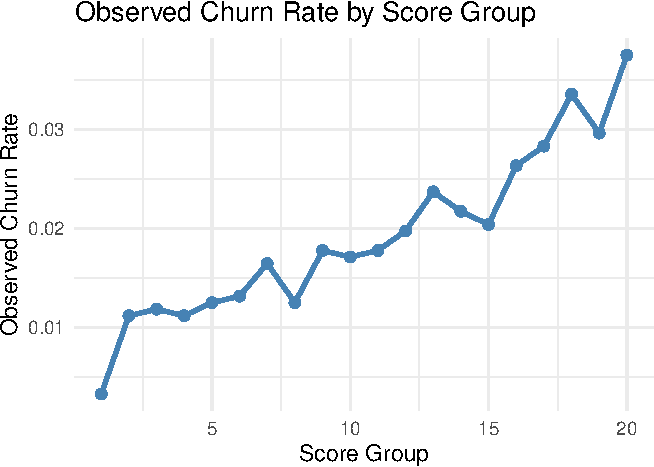
\includegraphics{p5-6_files/figure-latex/unnamed-chunk-14-1} \end{flushright}

\begin{Shaded}
\begin{Highlighting}[]
\CommentTok{\# Lift Factor vs. Score Groups}
\CommentTok{\# The lift factor should be highest for the top score groups (high{-}risk churners).}
\CommentTok{\# The horizontal line at y = 100 represents the baseline (random guessing or avg churn rate). }
\CommentTok{\# It hits close to the mid segment group reflects that the churn predictions align }
\CommentTok{\# with the reality (observation) of churn that is expected per each segment.}
\FunctionTok{ggplot}\NormalTok{(lift\_table, }\FunctionTok{aes}\NormalTok{(}\AttributeTok{x =}\NormalTok{ score\_group, }\AttributeTok{y =}\NormalTok{ lift\_factor)) }\SpecialCharTok{+}
  \FunctionTok{geom\_line}\NormalTok{(}\AttributeTok{color =} \StringTok{"darkorange"}\NormalTok{, }\AttributeTok{linewidth =} \DecValTok{1}\NormalTok{) }\SpecialCharTok{+}  \CommentTok{\# Use \textasciigrave{}linewidth\textasciigrave{} for line width}
  \FunctionTok{geom\_point}\NormalTok{(}\AttributeTok{color =} \StringTok{"darkorange"}\NormalTok{, }\AttributeTok{size =} \DecValTok{2}\NormalTok{) }\SpecialCharTok{+}  \CommentTok{\# Points on the line}
  \FunctionTok{geom\_hline}\NormalTok{(}\AttributeTok{yintercept =} \DecValTok{100}\NormalTok{, }\AttributeTok{color =} \StringTok{"red"}\NormalTok{, }\AttributeTok{linetype =} \StringTok{"dashed"}\NormalTok{) }\SpecialCharTok{+}  \CommentTok{\# Horizontal reference line}
  \FunctionTok{labs}\NormalTok{(}
    \AttributeTok{title =} \StringTok{"Lift Factor by Score Group"}\NormalTok{,}
    \AttributeTok{x =} \StringTok{"Score Group"}\NormalTok{,}
    \AttributeTok{y =} \StringTok{"Lift Factor"}
\NormalTok{  ) }\SpecialCharTok{+}
  \FunctionTok{theme\_minimal}\NormalTok{()}
\end{Highlighting}
\end{Shaded}

\begin{flushright}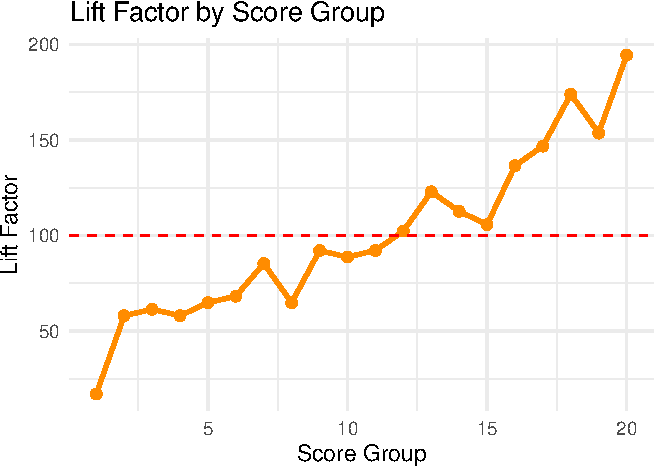
\includegraphics{p5-6_files/figure-latex/unnamed-chunk-14-2} \end{flushright}

\newpage

\section{Why do customers churn? --- Effect
sizes}\label{why-do-customers-churn-effect-sizes}

We would like to understand \emph{why} customers churn, which can help
us to propose incentives to prevent customer churn

\emph{To this end, construct a table that contains comparable effect
sizes (changes in the churn probability) for all independent variables,
as we discussed in class.}

Here are a few more details on the steps needed to create this table:

\begin{enumerate}
\def\labelenumi{\arabic{enumi}.}
\tightlist
\item
  Because logistic regression coefficients are not directly
  interpretable, we estimate a linear probability model of customer
  churn. In a linear probability model we regress the \(Y=0,1\) output
  on all the customer features. The estimated coefficients can be
  interpreted as differences in \(\Pr\{Y=1 | X_1, X_2, \dots\}\) for a
  one-unit difference in one of the features, \(X_k\). Note: \textbf{The
  \emph{offset variable} should not be included in the linear
  probability model as it is specific to logistic regression.}
\item
  Note that our analysis is based on a \emph{comparison} of the effect
  sizes of the different variables. However, because the variables have
  different scales, the effect sizes are not directly comparable. For
  example, \texttt{revenue} (mean monthly revenue) and \texttt{mou}
  (mean monthly minutes use) have different means and standard
  deviations, and hence the effects of increasing \texttt{revenue} and
  \texttt{mou} by one unit on the churn probabilities are not comparable
  without taking the scale differences into account.
\item
  To solve this problem we \textbf{standardize} the independent
  variables in the data. To standardize, we divide the values of each
  independent variable by its standard deviation, except if the variable
  is a 0/1 dummy. Once standardized, all variables except the dummies
  will have a standard deviation of 1, and a one unit difference
  corresponds to a one standard deviation difference in the original,
  non-standardized variable. Here's a function,
  \texttt{standardize\_columns}, that takes a column \texttt{x} as input
  and returns the standardized values of the column:
\end{enumerate}

\begin{Shaded}
\begin{Highlighting}[]
\NormalTok{standardize\_columns }\OtherTok{\textless{}{-}} \ControlFlowTok{function}\NormalTok{(x) \{}
   
   \CommentTok{\# Check if the column is a dummy variable}
\NormalTok{   elements }\OtherTok{=} \FunctionTok{unique}\NormalTok{(x)}
   \ControlFlowTok{if}\NormalTok{ (}\FunctionTok{length}\NormalTok{(elements) }\SpecialCharTok{==} \DecValTok{2}\DataTypeTok{L} \SpecialCharTok{\&} \FunctionTok{all}\NormalTok{(elements }\SpecialCharTok{\%in\%} \FunctionTok{c}\NormalTok{(}\DecValTok{0}\DataTypeTok{L}\NormalTok{,}\DecValTok{1}\DataTypeTok{L}\NormalTok{))) \{}
\NormalTok{      is\_dummy }\OtherTok{=} \ConstantTok{TRUE}
\NormalTok{   \} }\ControlFlowTok{else}\NormalTok{ \{}
\NormalTok{      is\_dummy }\OtherTok{=} \ConstantTok{FALSE}
\NormalTok{   \}}
   
   \CommentTok{\# If not a dummy, divide values in x by its standard deviation}
   \ControlFlowTok{if}\NormalTok{ (is\_dummy }\SpecialCharTok{==} \ConstantTok{FALSE}\NormalTok{) x }\OtherTok{=}\NormalTok{ x}\SpecialCharTok{/}\FunctionTok{sd}\NormalTok{(x, }\AttributeTok{na.rm =} \ConstantTok{TRUE}\NormalTok{)}
   
   \FunctionTok{return}\NormalTok{(x)}
\NormalTok{\}}
\end{Highlighting}
\end{Shaded}

The first part of the function checks that the input \texttt{x} has
exactly two elements and that these elements are the integers 0 and 1.
Note that in R, numbers are represented as floating point numbers by
default. However, adding \texttt{L} after the numbers tells R to
represent the number as an integer.

\begin{Shaded}
\begin{Highlighting}[]
\FunctionTok{class}\NormalTok{(}\DecValTok{1}\NormalTok{)}
\end{Highlighting}
\end{Shaded}

\begin{verbatim}
[1] "numeric"
\end{verbatim}

\begin{Shaded}
\begin{Highlighting}[]
\FunctionTok{class}\NormalTok{(}\DecValTok{1}\DataTypeTok{L}\NormalTok{)}
\end{Highlighting}
\end{Shaded}

\begin{verbatim}
[1] "integer"
\end{verbatim}

\begin{Shaded}
\begin{Highlighting}[]
\NormalTok{DT\_lin\_prob }\OtherTok{=}\NormalTok{ cell2cell\_clean[calibrat }\SpecialCharTok{==} \DecValTok{1}\NormalTok{]}

\CommentTok{\# Create a vector that contains the names of all inputs (covariates)}
\CommentTok{\# remove customer, calibrat, churn columns, retcall}
\NormalTok{all\_columns   }\OtherTok{=} \FunctionTok{names}\NormalTok{(DT\_lin\_prob)}
\NormalTok{input\_columns }\OtherTok{=}\NormalTok{ all\_columns[}\SpecialCharTok{{-}}\FunctionTok{c}\NormalTok{(}\DecValTok{1}\SpecialCharTok{:}\DecValTok{3}\NormalTok{, }\FunctionTok{length}\NormalTok{(all\_columns))] }

\CommentTok{\# Standardize all input columns}
\NormalTok{DT\_lin\_prob[, (input\_columns) }\SpecialCharTok{:=} \FunctionTok{lapply}\NormalTok{(.SD, standardize\_columns), .SDcols }\OtherTok{=}\NormalTok{ input\_columns]}

\FunctionTok{library}\NormalTok{(tidyverse)}

\NormalTok{Dv\_lin\_prob }\OtherTok{=}\NormalTok{ cell2cell\_clean[calibrat }\SpecialCharTok{==} \DecValTok{0}\NormalTok{]}

\CommentTok{\# Create a vector that contains the names of all inputs (covariates)}
\NormalTok{all\_columns   }\OtherTok{=} \FunctionTok{names}\NormalTok{(Dv\_lin\_prob)}
\NormalTok{input\_columns }\OtherTok{=}\NormalTok{ all\_columns[}\SpecialCharTok{{-}}\FunctionTok{c}\NormalTok{(}\DecValTok{1}\SpecialCharTok{:}\DecValTok{3}\NormalTok{, }\FunctionTok{length}\NormalTok{(all\_columns))]}

\CommentTok{\# Standardize all input columns}
\NormalTok{Dv\_lin\_prob[, (input\_columns) }\SpecialCharTok{:=} \FunctionTok{lapply}\NormalTok{(.SD, standardize\_columns), .SDcols }\OtherTok{=}\NormalTok{ input\_columns]}

\CommentTok{\# Calculate average churn probabilities in training and validation samples}
\NormalTok{avg\_churn\_train }\OtherTok{\textless{}{-}} \FunctionTok{mean}\NormalTok{(DT\_lin\_prob}\SpecialCharTok{$}\NormalTok{churn)}
\NormalTok{avg\_churn\_valid }\OtherTok{\textless{}{-}} \FunctionTok{mean}\NormalTok{(Dv\_lin\_prob}\SpecialCharTok{$}\NormalTok{churn)}

\CommentTok{\# Specify the formula excluding the first three columns}
\NormalTok{independent\_vars }\OtherTok{=} \FunctionTok{names}\NormalTok{(DT\_lin\_prob)[}\SpecialCharTok{{-}}\NormalTok{(}\DecValTok{1}\SpecialCharTok{:}\DecValTok{3}\NormalTok{)]}
\NormalTok{formula }\OtherTok{\textless{}{-}} \FunctionTok{as.formula}\NormalTok{(}\FunctionTok{paste}\NormalTok{(}\StringTok{"churn \textasciitilde{}"}\NormalTok{, }\FunctionTok{paste}\NormalTok{(independent\_vars, }\AttributeTok{collapse =} \StringTok{" + "}\NormalTok{)))}

\CommentTok{\# Fit the lpm model}
\NormalTok{lm\_model }\OtherTok{\textless{}{-}} \FunctionTok{lm}\NormalTok{(formula, }\AttributeTok{data =}\NormalTok{ cell2cell\_clean, }\AttributeTok{family =} \StringTok{"binomial"}\NormalTok{)}
\end{Highlighting}
\end{Shaded}

\begin{verbatim}
Warning: In lm.fit(x, y, offset = offset, singular.ok = singular.ok, ...) :
 extra argument 'family' will be disregarded
\end{verbatim}

\begin{Shaded}
\begin{Highlighting}[]
\CommentTok{\# Tidy the linear probability model output}
\NormalTok{tidy\_model }\OtherTok{\textless{}{-}} \FunctionTok{tidy}\NormalTok{(lm\_model)}

\CommentTok{\# Add effect\_size column}
\NormalTok{tidy\_model }\OtherTok{\textless{}{-}}\NormalTok{ tidy\_model }\SpecialCharTok{\%\textgreater{}\%}
  \FunctionTok{mutate}\NormalTok{(}\AttributeTok{effect\_size =}\NormalTok{ estimate }\SpecialCharTok{*}\NormalTok{ (}\DecValTok{100} \SpecialCharTok{*}\NormalTok{ avg\_churn\_valid }\SpecialCharTok{/}\NormalTok{ avg\_churn\_train))}

\CommentTok{\# Sort by absolute effect\_size and print the table}
\NormalTok{tidy\_model }\OtherTok{\textless{}{-}}\NormalTok{ tidy\_model }\SpecialCharTok{\%\textgreater{}\%} \FunctionTok{arrange}\NormalTok{(}\FunctionTok{desc}\NormalTok{(}\FunctionTok{abs}\NormalTok{(effect\_size)))}
\FunctionTok{kable}\NormalTok{(tidy\_model)}
\end{Highlighting}
\end{Shaded}

\begin{longtable}[]{@{}
  >{\raggedright\arraybackslash}p{(\columnwidth - 10\tabcolsep) * \real{0.1791}}
  >{\raggedleft\arraybackslash}p{(\columnwidth - 10\tabcolsep) * \real{0.1642}}
  >{\raggedleft\arraybackslash}p{(\columnwidth - 10\tabcolsep) * \real{0.1493}}
  >{\raggedleft\arraybackslash}p{(\columnwidth - 10\tabcolsep) * \real{0.1791}}
  >{\raggedleft\arraybackslash}p{(\columnwidth - 10\tabcolsep) * \real{0.1493}}
  >{\raggedleft\arraybackslash}p{(\columnwidth - 10\tabcolsep) * \real{0.1791}}@{}}
\toprule\noalign{}
\begin{minipage}[b]{\linewidth}\raggedright
term
\end{minipage} & \begin{minipage}[b]{\linewidth}\raggedleft
estimate
\end{minipage} & \begin{minipage}[b]{\linewidth}\raggedleft
std.error
\end{minipage} & \begin{minipage}[b]{\linewidth}\raggedleft
statistic
\end{minipage} & \begin{minipage}[b]{\linewidth}\raggedleft
p.value
\end{minipage} & \begin{minipage}[b]{\linewidth}\raggedleft
effect\_size
\end{minipage} \\
\midrule\noalign{}
\endhead
\bottomrule\noalign{}
\endlastfoot
(Intercept) & 0.3155318 & 0.0154054 & 20.4819562 & 0.0000000 &
1.2222911 \\
retcall & 0.1428622 & 0.0334030 & 4.2769308 & 0.0000190 & 0.5534125 \\
creditaa & -0.0746562 & 0.0054187 & -13.7775804 & 0.0000000 &
-0.2891994 \\
refurb & 0.0497153 & 0.0052670 & 9.4389822 & 0.0000000 & 0.1925846 \\
retaccpt & -0.0454461 & 0.0180450 & -2.5184894 & 0.0117882 &
-0.1760470 \\
retcalls & 0.0436851 & 0.0318359 & 1.3721972 & 0.1700065 & 0.1692253 \\
credita & -0.0374406 & 0.0057344 & -6.5290790 & 0.0000000 &
-0.1450354 \\
webcap & -0.0325533 & 0.0062916 & -5.1741180 & 0.0000002 & -0.1261035 \\
actvsubs & -0.0260920 & 0.0042041 & -6.2063671 & 0.0000000 &
-0.1010739 \\
occhmkr & 0.0255888 & 0.0300500 & 0.8515430 & 0.3944707 & 0.0991247 \\
prizmrur & 0.0251413 & 0.0082316 & 3.0542525 & 0.0022571 & 0.0973913 \\
children & 0.0219170 & 0.0045942 & 4.7705388 & 0.0000018 & 0.0849008 \\
uniqsubs & 0.0216580 & 0.0023639 & 9.1619086 & 0.0000000 & 0.0838977 \\
marryun & 0.0184553 & 0.0055491 & 3.3258146 & 0.0008821 & 0.0714911 \\
mailres & -0.0182875 & 0.0139969 & -1.3065363 & 0.1913746 &
-0.0708411 \\
mcycle & 0.0179938 & 0.0147568 & 1.2193553 & 0.2227135 & 0.0697033 \\
setprcm & -0.0179207 & 0.0065143 & -2.7509916 & 0.0059431 &
-0.0694203 \\
refer & -0.0164161 & 0.0065690 & -2.4990389 & 0.0124554 & -0.0635920 \\
creditcd & 0.0162241 & 0.0069966 & 2.3188679 & 0.0204051 & 0.0628480 \\
occcler & 0.0159186 & 0.0122084 & 1.3038995 & 0.1922722 & 0.0616646 \\
occstud & 0.0150096 & 0.0195761 & 0.7667340 & 0.4432423 & 0.0581436 \\
incmiss & -0.0137615 & 0.0097467 & -1.4119094 & 0.1579811 &
-0.0533085 \\
marryyes & 0.0109617 & 0.0052656 & 2.0817593 & 0.0373681 & 0.0424629 \\
occret & -0.0107438 & 0.0146348 & -0.7341284 & 0.4628730 & -0.0416190 \\
prizmtwn & 0.0099962 & 0.0051531 & 1.9398633 & 0.0524004 & 0.0387229 \\
phones & 0.0091587 & 0.0028875 & 3.1718725 & 0.0015153 & 0.0354785 \\
mailord & -0.0086711 & 0.0139311 & -0.6224300 & 0.5336612 &
-0.0335897 \\
ownrent & 0.0080209 & 0.0069890 & 1.1476508 & 0.2511167 & 0.0310710 \\
newcelly & -0.0068243 & 0.0044463 & -1.5348272 & 0.1248309 &
-0.0264356 \\
newcelln & 0.0067779 & 0.0051506 & 1.3159517 & 0.1881946 & 0.0262560 \\
prizmub & -0.0065886 & 0.0039796 & -1.6555940 & 0.0978086 &
-0.0255224 \\
truck & 0.0061767 & 0.0058655 & 1.0530690 & 0.2923130 & 0.0239271 \\
occcrft & -0.0058655 & 0.0102090 & -0.5745377 & 0.5656058 &
-0.0227213 \\
threeway & -0.0056046 & 0.0015879 & -3.5296127 & 0.0004164 &
-0.0217107 \\
pcown & 0.0046355 & 0.0050451 & 0.9188126 & 0.3581968 & 0.0179568 \\
months & -0.0039985 & 0.0003112 & -12.8490599 & 0.0000000 &
-0.0154893 \\
rv & 0.0032359 & 0.0078461 & 0.4124217 & 0.6800316 & 0.0125350 \\
models & 0.0030603 & 0.0044645 & 0.6854850 & 0.4930402 & 0.0118550 \\
occprof & -0.0028973 & 0.0052951 & -0.5471700 & 0.5842637 &
-0.0112236 \\
callfwdv & -0.0023206 & 0.0030577 & -0.7589262 & 0.4478993 &
-0.0089893 \\
occself & -0.0022278 & 0.0131317 & -0.1696487 & 0.8652869 &
-0.0086298 \\
mailflag & 0.0021229 & 0.0141718 & 0.1497977 & 0.8809247 & 0.0082236 \\
dropvce & 0.0015669 & 0.0013081 & 1.1978461 & 0.2309810 & 0.0060696 \\
income & -0.0013005 & 0.0009818 & -1.3246965 & 0.1852762 & -0.0050380 \\
travel & 0.0011499 & 0.0077021 & 0.1493014 & 0.8813163 & 0.0044545 \\
custcare & -0.0009738 & 0.0003752 & -2.5958113 & 0.0094388 &
-0.0037724 \\
age1 & -0.0008056 & 0.0001416 & -5.6910243 & 0.0000000 & -0.0031208 \\
blckvce & 0.0006473 & 0.0012956 & 0.4995951 & 0.6173618 & 0.0025074 \\
recchrge & -0.0005385 & 0.0001443 & -3.7308807 & 0.0001910 &
-0.0020861 \\
roam & 0.0005263 & 0.0002299 & 2.2892024 & 0.0220706 & 0.0020389 \\
changer & 0.0005231 & 0.0000555 & 9.4178059 & 0.0000000 & 0.0020265 \\
revenue & 0.0003348 & 0.0001279 & 2.6177138 & 0.0088540 & 0.0012970 \\
eqpdays & 0.0002750 & 0.0000118 & 23.3543418 & 0.0000000 & 0.0010653 \\
incalls & -0.0002686 & 0.0001654 & -1.6240220 & 0.1043757 &
-0.0010404 \\
callwait & 0.0001829 & 0.0004725 & 0.3871468 & 0.6986487 & 0.0007086 \\
age2 & -0.0001770 & 0.0001100 & -1.6091271 & 0.1075931 & -0.0006856 \\
overage & 0.0001579 & 0.0000451 & 3.4999792 & 0.0004656 & 0.0006116 \\
unansvce & 0.0001527 & 0.0000705 & 2.1647194 & 0.0304126 & 0.0005914 \\
peakvce & -0.0001153 & 0.0000345 & -3.3417639 & 0.0008329 &
-0.0004468 \\
outcalls & 0.0001038 & 0.0000917 & 1.1319893 & 0.2576429 & 0.0004021 \\
changem & -0.0001028 & 0.0000085 & -12.0987909 & 0.0000000 &
-0.0003981 \\
setprc & 0.0000899 & 0.0000454 & 1.9797035 & 0.0477408 & 0.0003482 \\
mou & -0.0000508 & 0.0000080 & -6.3614191 & 0.0000000 & -0.0001970 \\
opeakvce & -0.0000471 & 0.0000416 & -1.1318473 & 0.2577025 &
-0.0001824 \\
dropblk & -0.0000304 & 0.0012767 & -0.0238423 & 0.9809785 &
-0.0001179 \\
mourec & 0.0000274 & 0.0000212 & 1.2945619 & 0.1954757 & 0.0001061 \\
directas & 0.0000122 & 0.0008945 & 0.0136384 & 0.9891185 & 0.0000473 \\
\end{longtable}

\begin{enumerate}
\def\labelenumi{\arabic{enumi}.}
\setcounter{enumi}{3}
\tightlist
\item
  In order to create a table that captures the linear probability model
  estimates, use the \texttt{tidy} function. Add a column, e.g.
  \texttt{effect\_size}, that scales the estimates by the factor
  \[100 \cdot \frac{\bar{p}_{v}}{\bar{p}_{t}}\] This scales the effect
  sizes to the correct magnitude of the churn probabilities in the
  validation sample and puts the effects on a 0-100\% scale. Sort the
  variables according to the magnitude of the effect sizes, and print
  the results table using \texttt{kable}.
\item
  Inspect the results. Identify some factors that are strongly
  associated with churn. If actionable, propose an incentive that can be
  targeted to the customers to prevent churn.
\end{enumerate}

\begin{Shaded}
\begin{Highlighting}[]
\NormalTok{sorted\_model }\OtherTok{\textless{}{-}}\NormalTok{ tidy\_model }\SpecialCharTok{\%\textgreater{}\%} \FunctionTok{arrange}\NormalTok{(}\FunctionTok{desc}\NormalTok{(effect\_size))}
\NormalTok{top\_5 }\OtherTok{\textless{}{-}} \FunctionTok{head}\NormalTok{(sorted\_model, }\DecValTok{5}\NormalTok{)}
\NormalTok{bottom\_5 }\OtherTok{\textless{}{-}} \FunctionTok{tail}\NormalTok{(sorted\_model, }\DecValTok{5}\NormalTok{)}

\FunctionTok{print}\NormalTok{(top\_5)}
\end{Highlighting}
\end{Shaded}

\begin{verbatim}
# A tibble: 5 x 6
  term        estimate std.error statistic  p.value effect_size
  <chr>          <dbl>     <dbl>     <dbl>    <dbl>       <dbl>
1 (Intercept)   0.316    0.0154     20.5   5.89e-93      1.22  
2 retcall       0.143    0.0334      4.28  1.90e- 5      0.553 
3 refurb        0.0497   0.00527     9.44  3.88e-21      0.193 
4 retcalls      0.0437   0.0318      1.37  1.70e- 1      0.169 
5 occhmkr       0.0256   0.0300      0.852 3.94e- 1      0.0991
\end{verbatim}

\begin{Shaded}
\begin{Highlighting}[]
\FunctionTok{print}\NormalTok{(bottom\_5)}
\end{Highlighting}
\end{Shaded}

\begin{verbatim}
# A tibble: 5 x 6
  term     estimate std.error statistic  p.value effect_size
  <chr>       <dbl>     <dbl>     <dbl>    <dbl>       <dbl>
1 actvsubs  -0.0261   0.00420     -6.21 5.45e-10      -0.101
2 webcap    -0.0326   0.00629     -5.17 2.30e- 7      -0.126
3 credita   -0.0374   0.00573     -6.53 6.66e-11      -0.145
4 retaccpt  -0.0454   0.0180      -2.52 1.18e- 2      -0.176
5 creditaa  -0.0747   0.00542    -13.8  3.96e-43      -0.289
\end{verbatim}

Factors that are strongly associated with churn. Strong positively churn
1. retcall (0.55341249) : Customers with retention calls are more likely
to churn, possibly due to dissatisfaction with previous interactions or
unresolved issues. Highly significant (p=1.89e-05) Incentive : -
Personalized Service Recovery: Provide dedicated, high-quality customer
service follow-ups for customers who have made a retention call,
ensuring their issues are fully resolved. - Offer discounts or credits
(e.g., one-time \$50 credit) for the inconvenience.

\begin{enumerate}
\def\labelenumi{\arabic{enumi}.}
\setcounter{enumi}{1}
\tightlist
\item
  refurb (0.19258463) : Customers with refurbished devices are more
  likely to churn, possibly due to dissatisfaction with older hardware.
  Highly significant(p=3.87e10-21) Incentive :
\end{enumerate}

\begin{itemize}
\tightlist
\item
  Upgrade Program : Create trade-in programs allowing refurbished users
  to easily swap for newer models at minimal cost.
\end{itemize}

\begin{enumerate}
\def\labelenumi{\arabic{enumi}.}
\setcounter{enumi}{2}
\tightlist
\item
  retcalls frequency (0.16922533) : Number of calls previously made to
  retention team, possibly due to dissatisfaction with the too frequent
  callings or unresolved issues. Incentive :
\end{enumerate}

\begin{itemize}
\tightlist
\item
  Implement a proactive monitoring system to identify frequent retention
  team callers and address their issues before they escalate.
\item
  Provide special discounts or perks (e.g., reduced fees for 3 months)
  to frequent retention callers to demonstrate appreciation and regain
  trust.
\end{itemize}

\begin{enumerate}
\def\labelenumi{\arabic{enumi}.}
\setcounter{enumi}{3}
\tightlist
\item
  occhmkr (0.09912475) : Occupation - homemaker are likely to churn,
  potentially due to higher demands for quality of product or services.
  Incentive :
\end{enumerate}

\begin{itemize}
\tightlist
\item
  Introduce a family-oriented subscription plans with better value for
  households.
\item
  Offer special perks for homemakers.
\end{itemize}

Strong negatively churn (unlikely to churn) 1. creditaa (-0.2891994) :
Customers with excellent credit ratings `aa' are less likely to churn,
possibly indicating higher satisfaction or loyalty. Incentive : - Offer
loyalty programs, such as discounts on premium services or free
upgrades, for customers who meet certain payment and credit score
thresholds.

\begin{enumerate}
\def\labelenumi{\arabic{enumi}.}
\setcounter{enumi}{1}
\tightlist
\item
  retaccpt (-0.1760470) : Customers who accept retention offers are less
  likely to churn, highlighting the effectiveness of these
  interventions. Incentive :
\end{enumerate}

\begin{itemize}
\tightlist
\item
  Post retention engagement : Provide incentives for continued loyalty,
  such as bonus points or exclusive access to new features.
\end{itemize}

\begin{enumerate}
\def\labelenumi{\arabic{enumi}.}
\setcounter{enumi}{2}
\tightlist
\item
  credita (-0.1450354) : Customers with excellent credit ratings `a' are
  less likely to churn. Similar to creditaa. Incentive :
\end{enumerate}

\begin{itemize}
\tightlist
\item
  Send message to encourage them to earn more points to move to the `aa'
  tier.
\end{itemize}

\newpage

\section{Economics of churn
management}\label{economics-of-churn-management}

Next, we would like to predict the value of a proposed churn management
program in order to assess the maximum amount that we would spend to
prevent a customer from churning for one year.

\emph{Perform this prediction}, under the following assumptions:

\begin{enumerate}
\def\labelenumi{\arabic{enumi}.}
\tightlist
\item
  We consider a planning horizon of 4 years (the current year and three
  additional years), and an annual discount rate of 8 percent.
\item
  Predict the churn management value for 20 groups, but keep in mind
  that it is good practice to make sure the code works for an arbitrary
  number of groups in case we wish to modify that in the future. Predict
  the program value for these 20 customer segments based on the
  predicted churn rate. Note that we create these segments based on the
  validation sample data. We predict current and future customer profits
  at the year-level. Hence, we also need to convert both the monthly
  churn rate and the revenue data to the year-level.
\item
  Assume that the churn management program has a success probability
  \texttt{gamma} (\(\gamma\)) and compare the results for
  \(\gamma=0.25\) and \(\gamma=0.5\).
\end{enumerate}

\medskip

Hint: It is easy to make little mistakes in the lifetime value
predictions. Hence, be very clear about what your code is supposed to
achieve, and check that every step is correct.

\begin{Shaded}
\begin{Highlighting}[]
\CommentTok{\# Program Value }
\CommentTok{\# Gamma = 0.25 : Adjusted LTV for success probability 25\%.}
\CommentTok{\# Gamma = 0.50 : Adjusted LTV for success probability 50\%.}

\CommentTok{\# Parameters}
\NormalTok{discount\_rate }\OtherTok{\textless{}{-}} \FloatTok{0.08}
\NormalTok{gamma\_values }\OtherTok{\textless{}{-}} \FunctionTok{c}\NormalTok{(}\FloatTok{0.25}\NormalTok{, }\FloatTok{0.5}\NormalTok{)}
\NormalTok{groups }\OtherTok{\textless{}{-}} \DecValTok{20}
\NormalTok{horizon }\OtherTok{\textless{}{-}} \DecValTok{4}  \CommentTok{\# 4 years}

\CommentTok{\# Convert monthly churn rate and revenue to yearly}
\NormalTok{validation\_data }\OtherTok{\textless{}{-}}\NormalTok{ validation\_sample }
\NormalTok{validation\_data[, churn\_rate\_yearly }\SpecialCharTok{:=} \DecValTok{1} \SpecialCharTok{{-}}\NormalTok{ (}\DecValTok{1} \SpecialCharTok{{-}}\NormalTok{ predicted\_churn)}\SpecialCharTok{\^{}}\DecValTok{12}\NormalTok{]}
\NormalTok{validation\_data[, revenue\_yearly }\SpecialCharTok{:=}\NormalTok{ revenue }\SpecialCharTok{*} \DecValTok{12}\NormalTok{]}

\CommentTok{\# Group data into segments }
\CommentTok{\# The segment is in the score\_group column}
\NormalTok{validation\_data[, score\_group }\SpecialCharTok{:=} \FunctionTok{as.integer}\NormalTok{(}\FunctionTok{cut\_number}\NormalTok{(predicted\_churn, }\AttributeTok{n =}\NormalTok{ groups))]}

\CommentTok{\# Function to calculate LTV}
\NormalTok{calculate\_ltv }\OtherTok{\textless{}{-}} \ControlFlowTok{function}\NormalTok{(revenue, churn\_rate, discount\_rate, horizon) \{}
\NormalTok{  ltv }\OtherTok{\textless{}{-}} \DecValTok{0}
  \ControlFlowTok{for}\NormalTok{ (t }\ControlFlowTok{in} \DecValTok{0}\SpecialCharTok{:}\NormalTok{(horizon }\SpecialCharTok{{-}} \DecValTok{1}\NormalTok{)) \{}
\NormalTok{    ltv }\OtherTok{\textless{}{-}}\NormalTok{ ltv }\SpecialCharTok{+}\NormalTok{ (revenue }\SpecialCharTok{*}\NormalTok{ (}\DecValTok{1} \SpecialCharTok{{-}}\NormalTok{ churn\_rate)}\SpecialCharTok{\^{}}\NormalTok{t) }\SpecialCharTok{/}\NormalTok{ ((}\DecValTok{1} \SpecialCharTok{+}\NormalTok{ discount\_rate)}\SpecialCharTok{\^{}}\NormalTok{t)}
\NormalTok{  \}}
  \FunctionTok{return}\NormalTok{(ltv)}
\NormalTok{\}}
\end{Highlighting}
\end{Shaded}

\begin{Shaded}
\begin{Highlighting}[]
\CommentTok{\# Calculate metrics for each group}
\NormalTok{group\_summary }\OtherTok{\textless{}{-}}\NormalTok{ validation\_data[, .(}
  \AttributeTok{num\_customers =}\NormalTok{ .N,  }\CommentTok{\# Count the number of rows (customers) in each group}
  \AttributeTok{avg\_churn\_rate =} \FunctionTok{mean}\NormalTok{(churn\_rate\_yearly),}
  \AttributeTok{avg\_revenue =} \FunctionTok{mean}\NormalTok{(revenue\_yearly),}
  \AttributeTok{avg\_ltv =} \FunctionTok{calculate\_ltv}\NormalTok{(}\FunctionTok{mean}\NormalTok{(revenue\_yearly), }\FunctionTok{mean}\NormalTok{(churn\_rate\_yearly), }
\NormalTok{                          discount\_rate, horizon)}
\NormalTok{  ), by }\OtherTok{=}\NormalTok{ score\_group]}

\CommentTok{\# Add program values for different success probabilities}
\CommentTok{\# If gamma = 0.25, the program is expected to succeed for 25\% of the customers it }
\CommentTok{\# targets,so only 25\% of the LTV is realized.}
\CommentTok{\# Program value shows the expected realized benefit}
\NormalTok{group\_summary[, program\_value\_gamma\_0}\FloatTok{.25} \SpecialCharTok{:=} \FloatTok{0.25} \SpecialCharTok{*}\NormalTok{ avg\_ltv]}
\NormalTok{group\_summary[, program\_value\_gamma\_0}\FloatTok{.5} \SpecialCharTok{:=} \FloatTok{0.5} \SpecialCharTok{*}\NormalTok{ avg\_ltv]}

\CommentTok{\# Add max\_spend per each program to the table}
\NormalTok{group\_summary[, max\_spend\_gamma\_0}\FloatTok{.25} \SpecialCharTok{:=}\NormalTok{ program\_value\_gamma\_0}\FloatTok{.25} \SpecialCharTok{/}\NormalTok{ horizon]}
\NormalTok{group\_summary[, max\_spend\_gamma\_0}\FloatTok{.5} \SpecialCharTok{:=}\NormalTok{ program\_value\_gamma\_0}\FloatTok{.5} \SpecialCharTok{/}\NormalTok{ horizon]}
\NormalTok{group\_summary }\OtherTok{\textless{}{-}}\NormalTok{ group\_summary[}\FunctionTok{order}\NormalTok{(score\_group)]}

\NormalTok{group\_summary[, total\_program\_value\_gamma\_0}\FloatTok{.5} \SpecialCharTok{:=}\NormalTok{ max\_spend\_gamma\_0}\FloatTok{.5} \SpecialCharTok{*}\NormalTok{ num\_customers]}
\NormalTok{group\_summary[, total\_program\_value\_gamma\_0}\FloatTok{.25} \SpecialCharTok{:=}\NormalTok{ max\_spend\_gamma\_0}\FloatTok{.25} \SpecialCharTok{*}\NormalTok{ num\_customers]}

\CommentTok{\# View the updated table}
\FunctionTok{kable}\NormalTok{(group\_summary[, }\DecValTok{1}\SpecialCharTok{:}\DecValTok{7}\NormalTok{], }\AttributeTok{digits =} \DecValTok{2}\NormalTok{) }\SpecialCharTok{\%\textgreater{}\%}
  \FunctionTok{kable\_styling}\NormalTok{(}\AttributeTok{font\_size =} \DecValTok{8}\NormalTok{) }
\end{Highlighting}
\end{Shaded}

\begingroup\fontsize{8}{10}\selectfont

\begin{longtable}[t]{rrrrrrr}
\toprule
score\_group & num\_customers & avg\_churn\_rate & avg\_revenue & avg\_ltv & program\_value\_gamma\_0.25 & program\_value\_gamma\_0.5\\
\midrule
1 & 1519 & 0.08 & 1033.05 & 3279.97 & 819.99 & 1639.99\\
2 & 1518 & 0.11 & 845.28 & 2585.54 & 646.38 & 1292.77\\
3 & 1519 & 0.13 & 821.25 & 2460.57 & 615.14 & 1230.28\\
4 & 1518 & 0.14 & 764.15 & 2249.57 & 562.39 & 1124.79\\
5 & 1518 & 0.15 & 731.57 & 2122.20 & 530.55 & 1061.10\\
\addlinespace
6 & 1519 & 0.16 & 690.73 & 1977.92 & 494.48 & 988.96\\
7 & 1518 & 0.17 & 685.86 & 1941.09 & 485.27 & 970.55\\
8 & 1518 & 0.17 & 660.22 & 1847.54 & 461.89 & 923.77\\
9 & 1519 & 0.18 & 636.39 & 1761.43 & 440.36 & 880.71\\
10 & 1518 & 0.19 & 637.45 & 1744.94 & 436.24 & 872.47\\
\addlinespace
11 & 1518 & 0.20 & 664.12 & 1797.23 & 449.31 & 898.61\\
12 & 1519 & 0.21 & 626.87 & 1675.94 & 418.98 & 837.97\\
13 & 1518 & 0.21 & 623.76 & 1646.35 & 411.59 & 823.18\\
14 & 1518 & 0.22 & 640.54 & 1667.42 & 416.86 & 833.71\\
15 & 1519 & 0.24 & 648.65 & 1662.94 & 415.73 & 831.47\\
\addlinespace
16 & 1518 & 0.25 & 645.78 & 1625.52 & 406.38 & 812.76\\
17 & 1518 & 0.27 & 625.23 & 1537.26 & 384.32 & 768.63\\
18 & 1519 & 0.29 & 637.67 & 1521.07 & 380.27 & 760.53\\
19 & 1518 & 0.32 & 696.42 & 1586.37 & 396.59 & 793.18\\
20 & 1519 & 0.42 & 856.16 & 1695.42 & 423.85 & 847.71\\
\bottomrule
\end{longtable}
\endgroup{}

\begin{Shaded}
\begin{Highlighting}[]
\FunctionTok{kable}\NormalTok{(group\_summary[, }\DecValTok{8}\SpecialCharTok{:}\FunctionTok{ncol}\NormalTok{(group\_summary)], }\AttributeTok{digits =} \DecValTok{2}\NormalTok{) }\SpecialCharTok{\%\textgreater{}\%}
  \FunctionTok{kable\_styling}\NormalTok{(}\AttributeTok{font\_size =} \DecValTok{8}\NormalTok{)}
\end{Highlighting}
\end{Shaded}

\begingroup\fontsize{8}{10}\selectfont

\begin{longtable}[t]{rrrr}
\toprule
max\_spend\_gamma\_0.25 & max\_spend\_gamma\_0.5 & total\_program\_value\_gamma\_0.5 & total\_program\_value\_gamma\_0.25\\
\midrule
205.00 & 410.00 & 622784.5 & 311392.2\\
161.60 & 323.19 & 490605.7 & 245302.8\\
153.79 & 307.57 & 467200.5 & 233600.2\\
140.60 & 281.20 & 426856.8 & 213428.4\\
132.64 & 265.27 & 402686.9 & 201343.5\\
\addlinespace
123.62 & 247.24 & 375558.0 & 187779.0\\
121.32 & 242.64 & 368321.9 & 184160.9\\
115.47 & 230.94 & 350571.3 & 175285.7\\
110.09 & 220.18 & 334450.8 & 167225.4\\
109.06 & 218.12 & 331102.7 & 165551.3\\
\addlinespace
112.33 & 224.65 & 341024.3 & 170512.2\\
104.75 & 209.49 & 318219.0 & 159109.5\\
102.90 & 205.79 & 312395.8 & 156197.9\\
104.21 & 208.43 & 316393.7 & 158196.8\\
103.93 & 207.87 & 315749.8 & 157874.9\\
\addlinespace
101.59 & 203.19 & 308442.4 & 154221.2\\
96.08 & 192.16 & 291695.6 & 145847.8\\
95.07 & 190.13 & 288813.0 & 144406.5\\
99.15 & 198.30 & 301013.5 & 150506.7\\
105.96 & 211.93 & 321917.8 & 160958.9\\
\bottomrule
\end{longtable}
\endgroup{}

\begin{Shaded}
\begin{Highlighting}[]
\CommentTok{\# Select high{-}risk, high{-}value group to enter the program}

\CommentTok{\# Step 1: Filter for high{-}risk groups (avg\_churn\_rate \textgreater{} 0.2)}
\NormalTok{high\_risk\_groups }\OtherTok{\textless{}{-}}\NormalTok{ group\_summary[avg\_churn\_rate }\SpecialCharTok{\textgreater{}} \FloatTok{0.2}\NormalTok{]}

\CommentTok{\# Step 2: Prioritize by program value}
\NormalTok{prioritized\_groups }\OtherTok{\textless{}{-}}\NormalTok{ high\_risk\_groups[}\FunctionTok{order}\NormalTok{(}\SpecialCharTok{{-}}\NormalTok{program\_value\_gamma\_0}\FloatTok{.5}\NormalTok{)]}

\FunctionTok{kable}\NormalTok{(prioritized\_groups[, }\DecValTok{1}\SpecialCharTok{:}\DecValTok{7}\NormalTok{], }\AttributeTok{digits =} \DecValTok{2}\NormalTok{) }\SpecialCharTok{\%\textgreater{}\%}
  \FunctionTok{kable\_styling}\NormalTok{(}\AttributeTok{font\_size =} \DecValTok{8}\NormalTok{) }
\end{Highlighting}
\end{Shaded}

\begingroup\fontsize{8}{10}\selectfont

\begin{longtable}[t]{rrrrrrr}
\toprule
score\_group & num\_customers & avg\_churn\_rate & avg\_revenue & avg\_ltv & program\_value\_gamma\_0.25 & program\_value\_gamma\_0.5\\
\midrule
20 & 1519 & 0.42 & 856.16 & 1695.42 & 423.85 & 847.71\\
12 & 1519 & 0.21 & 626.87 & 1675.94 & 418.98 & 837.97\\
14 & 1518 & 0.22 & 640.54 & 1667.42 & 416.86 & 833.71\\
15 & 1519 & 0.24 & 648.65 & 1662.94 & 415.73 & 831.47\\
13 & 1518 & 0.21 & 623.76 & 1646.35 & 411.59 & 823.18\\
\addlinespace
16 & 1518 & 0.25 & 645.78 & 1625.52 & 406.38 & 812.76\\
19 & 1518 & 0.32 & 696.42 & 1586.37 & 396.59 & 793.18\\
17 & 1518 & 0.27 & 625.23 & 1537.26 & 384.32 & 768.63\\
18 & 1519 & 0.29 & 637.67 & 1521.07 & 380.27 & 760.53\\
\bottomrule
\end{longtable}
\endgroup{}

\begin{Shaded}
\begin{Highlighting}[]
\FunctionTok{kable}\NormalTok{(prioritized\_groups[, }\DecValTok{8}\SpecialCharTok{:}\FunctionTok{ncol}\NormalTok{(prioritized\_groups)], }\AttributeTok{digits =} \DecValTok{3}\NormalTok{) }\SpecialCharTok{\%\textgreater{}\%}
  \FunctionTok{kable\_styling}\NormalTok{(}\AttributeTok{font\_size =} \DecValTok{8}\NormalTok{)}
\end{Highlighting}
\end{Shaded}

\begingroup\fontsize{8}{10}\selectfont

\begin{longtable}[t]{rrrr}
\toprule
max\_spend\_gamma\_0.25 & max\_spend\_gamma\_0.5 & total\_program\_value\_gamma\_0.5 & total\_program\_value\_gamma\_0.25\\
\midrule
105.964 & 211.927 & 321917.8 & 160958.9\\
104.746 & 209.492 & 318219.0 & 159109.5\\
104.214 & 208.428 & 316393.7 & 158196.8\\
103.933 & 207.867 & 315749.8 & 157874.9\\
102.897 & 205.794 & 312395.8 & 156197.9\\
\addlinespace
101.595 & 203.190 & 308442.4 & 154221.2\\
99.148 & 198.296 & 301013.5 & 150506.7\\
96.079 & 192.158 & 291695.6 & 145847.8\\
95.067 & 190.134 & 288813.0 & 144406.5\\
\bottomrule
\end{longtable}
\endgroup{}

\begin{Shaded}
\begin{Highlighting}[]
\CommentTok{\# Find the Aggregate total max spending for the targeted group}


\CommentTok{\# Aggregate total max spend for gamma = 0.5}
\NormalTok{total\_program\_value\_gamma\_0}\FloatTok{.5} \OtherTok{\textless{}{-}} \FunctionTok{sum}\NormalTok{(prioritized\_groups}\SpecialCharTok{$}\NormalTok{total\_program\_value\_gamma\_0}\FloatTok{.5}\NormalTok{)}

\CommentTok{\# Aggregate total max spend for gamma = 0.25}
\NormalTok{total\_program\_value\_gamma\_0}\FloatTok{.25} \OtherTok{\textless{}{-}} \FunctionTok{sum}\NormalTok{(prioritized\_groups}\SpecialCharTok{$}\NormalTok{total\_program\_value\_gamma\_0}\FloatTok{.25}\NormalTok{)}

\FunctionTok{cat}\NormalTok{(}\StringTok{"Total max spend represents is the cumulative justification for running \textbackslash{}}
\StringTok{    the churn management program across all selected groups. }\SpecialCharTok{\textbackslash{}n}\StringTok{"}\NormalTok{)}
\end{Highlighting}
\end{Shaded}

\begin{verbatim}
Total max spend represents is the cumulative justification for running 
    the churn management program across all selected groups. 
\end{verbatim}

\begin{Shaded}
\begin{Highlighting}[]
\FunctionTok{cat}\NormalTok{(}\StringTok{"Total max spend for program (gamma = 0.5) \textbackslash{}}
\StringTok{    on selected group $"}\NormalTok{, }
\NormalTok{    total\_program\_value\_gamma\_0}\FloatTok{.5}\NormalTok{, }\StringTok{"per year. }\SpecialCharTok{\textbackslash{}n}\StringTok{"}\NormalTok{)}
\end{Highlighting}
\end{Shaded}

\begin{verbatim}
Total max spend for program (gamma = 0.5) 
    on selected group $ 2774641 per year. 
\end{verbatim}

\begin{Shaded}
\begin{Highlighting}[]
\FunctionTok{cat}\NormalTok{(}\StringTok{"Total max spend for program (gamma = 0.25) \textbackslash{}}
\StringTok{    on selected group $"}\NormalTok{, }
\NormalTok{    total\_program\_value\_gamma\_0}\FloatTok{.25}\NormalTok{, }\StringTok{"per year. }\SpecialCharTok{\textbackslash{}n}\StringTok{"}\NormalTok{)}
\end{Highlighting}
\end{Shaded}

\begin{verbatim}
Total max spend for program (gamma = 0.25) 
    on selected group $ 1387320 per year. 
\end{verbatim}

Analyzing Result :

Per segment

\begin{itemize}
\tightlist
\item
  For example, for score group 20, we can spend up to \$211.93 per
  customer per year, assuming a 50\% success probability (𝛾= 0.5 ).
\item
  For score group 20, we can spend up to \$105.96 per customer per year,
  assuming a 25\% success probability (𝛾= 0.25 ).
\end{itemize}

Per total

\begin{itemize}
\tightlist
\item
  `Total\_program\_value\_gamma\_0.5' column is indicating the total
  budget for each segment by taking into account of the number of
  customers.
\end{itemize}

Aggregate Sum on selected group

\begin{itemize}
\tightlist
\item
  Total max spend represents indicates the cumulative justification for
  running the churn management program across all selected groups. This
  is total budget we could allocate per each program.
\item
  Total max spend for program (gamma = 0.5) across selected group: \$
  2774641 per year. - Total max spend for program (gamma = 0.25) across
  selected group: \$ 1387320 per year.
\end{itemize}

\newpage

\section{Summarize your main results}\label{summarize-your-main-results}

\emph{Please organize your main results along the four questions posed
in the overview.}

\end{document}
